\documentclass[aspectratio=169]{beamer}

\usepackage[utf8]{inputenc}
\usetheme{Madrid}
\usecolortheme{beaver}

\usepackage{graphicx}
\graphicspath{ {./Resources/} }

% Title here
\title{SNUB, The SNHU Student Database}
\author{Tim, Ben, Joe, Max}
\institute{SNHU CS-114}

\begin{document}

\frame{\titlepage} % Draw the title page

\begin{frame}
    \frametitle{Features}

    
    \begin{block}{\centering C\# Was Used to Develop the Following Testing Environment:}
    \end{block}
    % Some columns
    \begin{columns}
        \begin{column}{0.3\textwidth}
            \begin{block}{Users are Directed to:}
            \begin{itemize}
                \item Connect to the server
                \item Select a class from a drop-down menu
                \item Select a note from the list box.
            \end{itemize}
            \end{block}
        \end{column}
        \begin{column}{0.48\textwidth}
            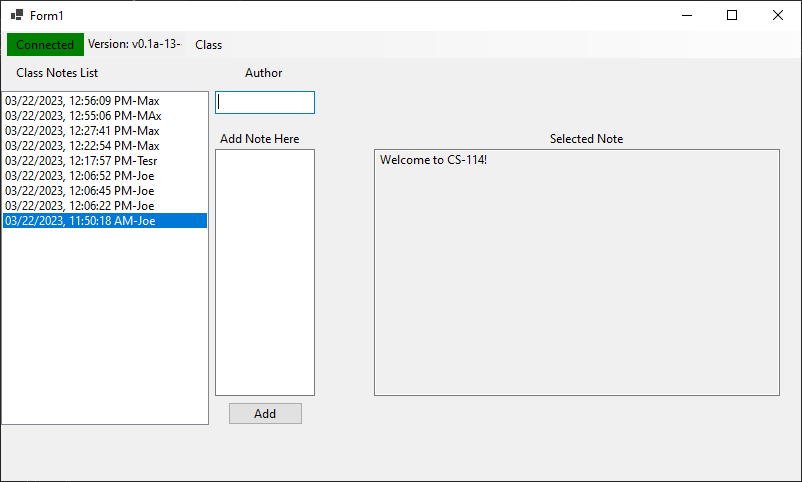
\includegraphics[width=8cm]{Sample_of_Features}
        \end{column}
    \end{columns}

\end{frame}

\begin{frame}
    \frametitle{Features}

    \begin{block}{\centering Connect to Server Feature}
        \centering 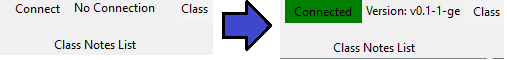
\includegraphics [width=9cm] {connect_to_connected.png}
    \end{block}
    \centering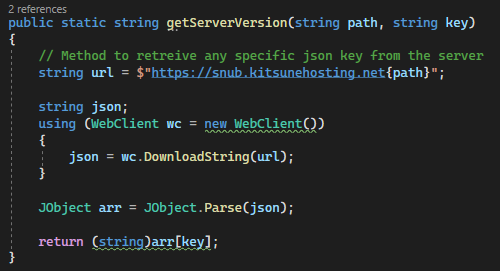
\includegraphics [width=9cm] {getServerVersion.PNG}
\end{frame}

\begin{frame}
    \frametitle{Features}

    \begin{block}{\centering Select a Class Feature}
        \centering Users are Directed to select a class from the drop-down menu. This populates the class notes list box with the date and author of each note corresponding to the selected class.
    \end{block}

    \centering 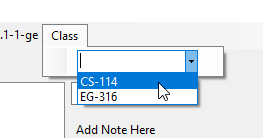
\includegraphics [width=10cm] {select}
    
\end{frame}

\begin{frame}
    \frametitle{Features}

    \begin{block}{\centering Populate Selected Note Feature}
        \centering Users may select an item from the list box to populate the selected note text box.
    \end{block}

    \centering 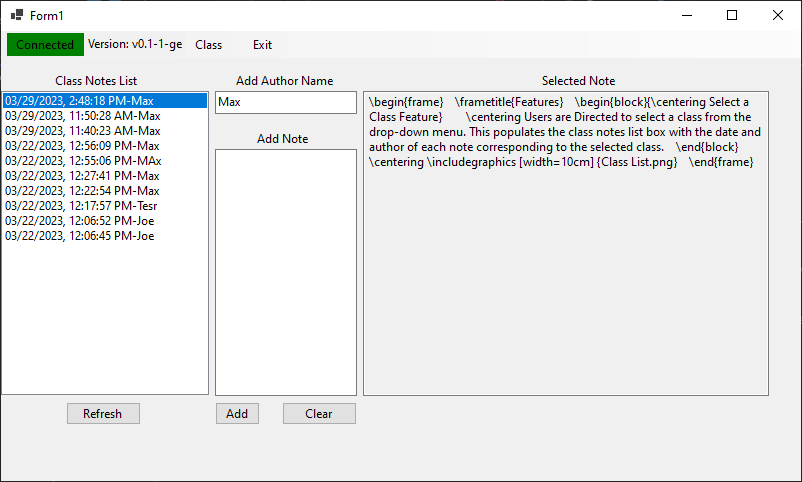
\includegraphics[height=5cm]{Select Class Note.png}
    
\end{frame}

\begin{frame}
    \frametitle{Features}

    \begin{block}{\centering Add Note Feature}
        \centering Users may add a note to the database by adding text to both the author and add note text boxes. If the user attempts to add a note containing an empty string they are prompted to try again.
    \end{block}

    \centering 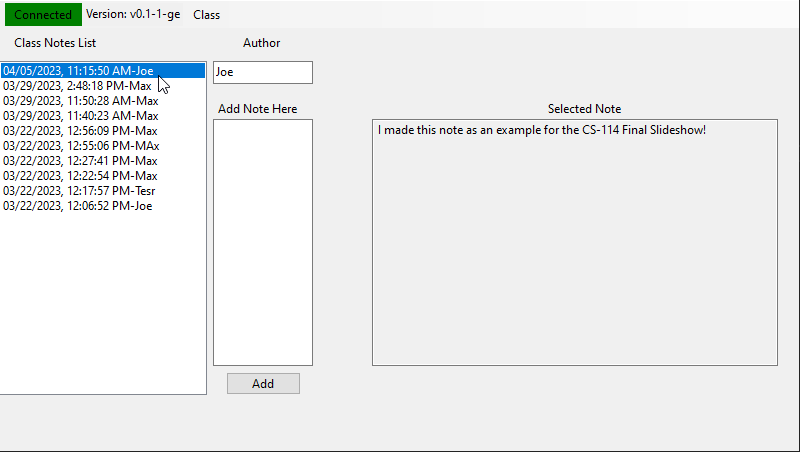
\includegraphics[height=5cm]{created.png}
\end{frame}

\begin{frame}
    \frametitle{Network and Database}

    % Some columns
    \begin{columns}
        \begin{column}{0.48\textwidth}
            \begin{block}{Data storage and Acquisition}
                All data is stored in a server, allowing for multiple clients. Data acquisition occurs as needed during use through a series of methods developed in c\#.
            \end{block}
        \end{column}
        \begin{column}{0.48\textwidth}
            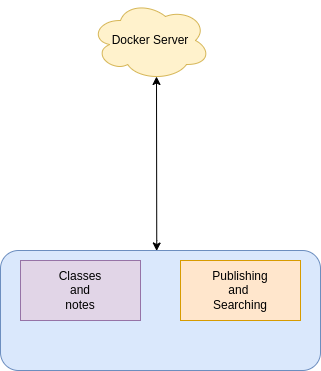
\includegraphics[width=5cm]{Simple Diagram.png}
        \end{column}
    \end{columns}
\end{frame}

\begin{frame}
    \frametitle{Github}

    % Some columns
    \begin{columns}
        \begin{column}{0.28\textwidth}
            \begin{block}{Github}
                We use github to build, check and publish both our docker images and the installer for our client.
            \end{block}
        \end{column}
        \begin{column}{0.58\textwidth}
            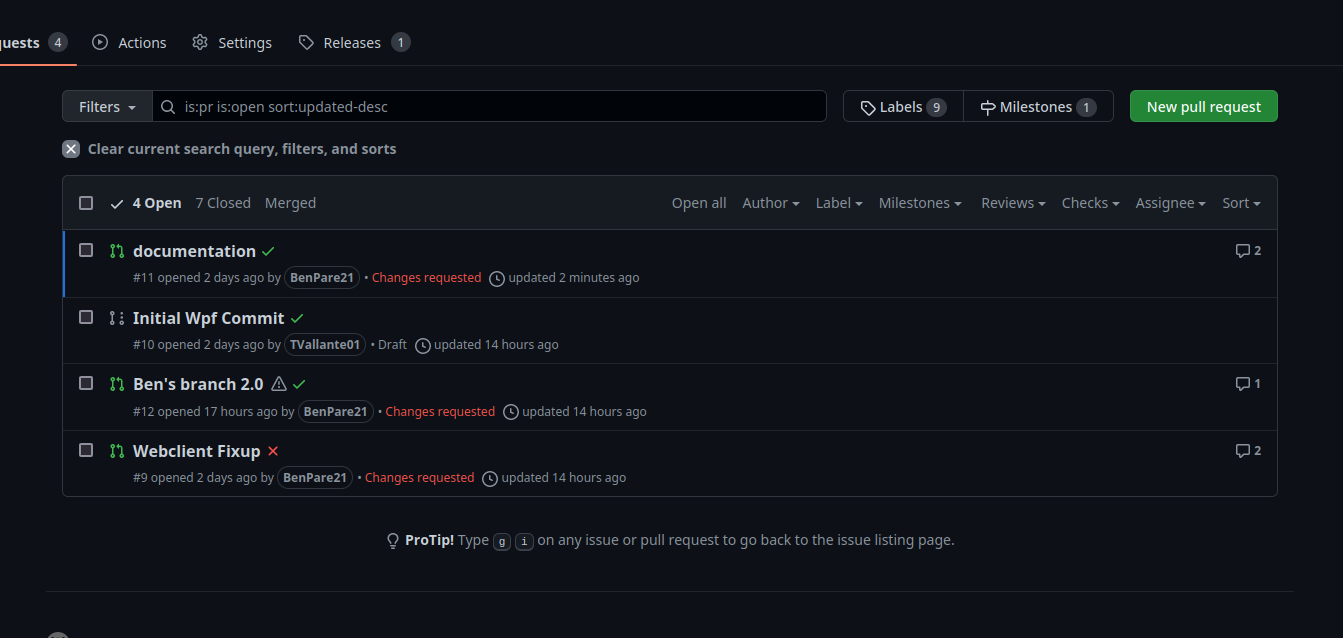
\includegraphics[width=9cm]{github.png}
        \end{column}
    \end{columns}
\end{frame}

\begin{frame}
    \frametitle{Alternative Clients}

    % Some columns
    \begin{columns}
        \begin{column}{0.38\textwidth}
            \begin{block}{WPF Client}
                Our unique server-side system allows for multiple different clients and a very even distribution of work.
            \end{block}
        \end{column}
        \begin{column}{0.58\textwidth}
            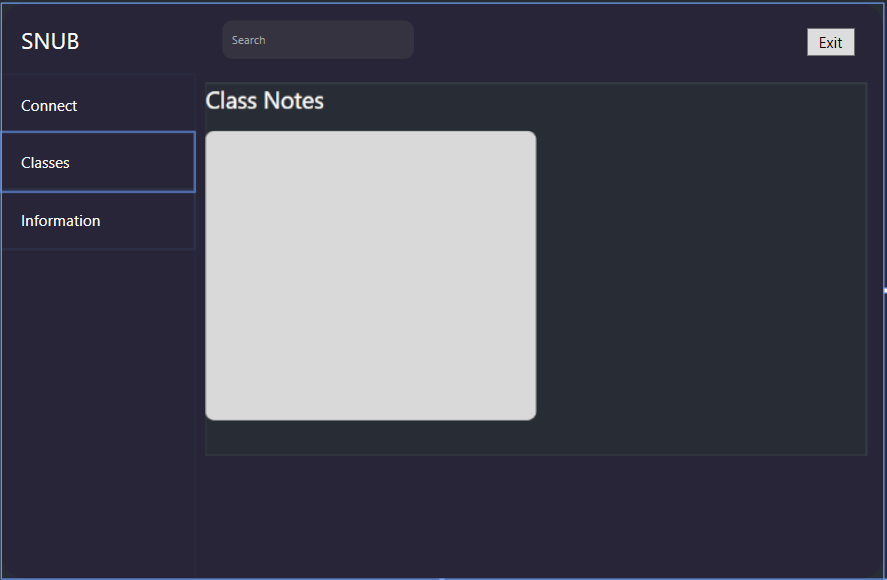
\includegraphics[width=9cm]{WpfBluePrint.png}
        \end{column}
    \end{columns}
\end{frame}

\begin{frame}
    \frametitle{End}

    \begin{block}{}
        \begin{center}
            \Huge Questions and Comments?
        \end{center}
    \end{block}

    \begin{center}
        Find the source code for this document, and the rest of our designs, firmware, hardware
        and notes on GitHub!

        
\includegraphics[height=4cm]{github_qr}
    \end{center}
\end{frame}

\end{document}

